\documentclass[a4paper,11pt,openright,oneside]{report}
\usepackage[utf8]{inputenc}
\usepackage[T1]{fontenc}
\usepackage[portuguese]{babel}
\usepackage{graphicx}
\usepackage[backend=biber, style=ieee]{biblatex}
\usepackage{csquotes}
\usepackage{blindtext}
\usepackage[printonlyused]{acronym}
\usepackage{hyperref}
\usepackage{minted}


\newcommand{\RNum}[1]{\uppercase\expandafter{\romannumeral #1\relax}}

\bibliography{biblio}

\begin{document}

\begin{titlepage}
\begin{center}

{\vspace*{50mm}\textsc{\Huge\textbf{Criptografia}\\ \small{Laboratórios de Informática}}}\\[2cm]
{\textsc{\small\textbf{Universidade de Aveiro}}}\\[0.5cm]
{\small Nelson Costa 42983\\Ricardo Jesus 76613}\\[0.5cm]
{\small	15 de Março de 2015}\\

\begin{figure}[b]
\center
\graphicspath{}

\includegraphics[height=2cm, width=2cm]{ua.pdf}
\end{figure}

\end{center}

\end{titlepage}

\title{\textbf{Criptografia}\\[1cm]\textsc{\small {Departamento de Electrónica, Telecomunicações e Informática} \\ \large {UNIVERSIDADE DE AVEIRO}}}
\author{Nelson Costa 42983, Ricardo Jesus 76613\\nelson.costa@ua.pt, ricardojesus@ua.pt}
\date{15 de Março de 2015}

\maketitle

\pagenumbering{roman}

\begin{abstract}



\end{abstract}

\tableofcontents
%\listoftables
\listoffigures

\clearpage
\pagenumbering{arabic}

\chapter{Introdução}
\label{chap.introdução}

\chapter{Criptografia}
\label{chap.criptografia}

A criptografia é a arte ou ciência de escrever uma mensagem de forma a ocultar o seu conteúdo. Dito por outras palavras, a criptografia usa técnicas que permitem que várias entidades possam transmitir mensagens de forma segura e privada, sem que estas sejam intercetadas e aproveitadas por terceiros. Independentemente do método que for usado para ocultar dados, a criptografia moderna pretende satisfazer 4 objetivos fundamentais:

\begin{description}
\item[Confidencialidade:] caso alguém intercetar a mensagem, essa pessoa não deve ser capaz de ler e perceber o seu conteúdo.
\item[Integridade dos dados:] o destinatário da mensagem deve ser capaz de verificar se a mensagem foi alterada durante a transmissão, acidental ou deliberadamente.
\item[Autenticação:] o destinatário da mensagem deve ser capaz de verificar a sua origem.
\item[Não-repúdio:] o remetente não deve ser capaz de negar mais tarde que foi realmente a pessoa que enviou a mensagem para o destinatário. O destinatário também não deve ser capaz de negar que recebeu a respetiva mensagem.
\end{description}
Existem alguns conceitos que são essenciais para a compreensão das operações envolvidas na criptografia. O termo cifra é o processo que transforma um texto em claro num texto cifrado ou geralmente chamado de criptograma. O termo decifra é a operação inversa da cifra, ou seja, transforma o criptograma no texto em claro original. As operações de cifra e decifra usam algoritmos e chaves, sendo estas utilizadas como parâmetros nos respetivos algoritmos. Os algoritmos são modelos matemáticos que contêm um conjunto de operações (ou regras) que permitem transformar os dados, ou seja, neste contexto, possibilita as operações de cifra e decifra. A figura \ref{fig:crypto0} mostra de forma simples os processos de cifra e decifra na criptografia.

\begin{figure}[ht]
\center
\fbox{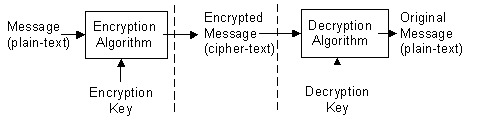
\includegraphics[height=3cm]{crypto0.jpg}}
\caption{Processos básicos de cifra e decifra na criptografia.}
\label{fig:crypto0}
\end{figure}

A mensagem original (plain-text) é cifrada usando um algoritmo e uma chave, produzindo uma mensagem cifrada (cipher-text). A mensagem cifrada é por sua vez decifrada usando um algoritmo e uma chave diferentes, obtendo-se a mensagem original (plain-text).

A criptografia pode ser dividida em várias áreas, entre os quais as criptografias simétrica, assimétrica e híbrida e as funções de síntese.

\section{Funções de Síntese}

Existem três tipos de algoritmos criptográficos: as chaves simétricas, assimétricas e as funções de síntese (Digest functions ou Hash functions). Ao contrário destas chaves, as funções de síntese não usam chaves. As funções de síntese produzem um valor de dimensão constante (hash value) a partir de um volume arbitrário de bits. Além disso, podem produzir valores diferentes para textos semelhantes. O principal objetivo destas funções na criptografia é a integridade dos dados. O valor que é produzido fornece uma impressão digital (Digital fingerprint) do conteúdo da mensagem, o que permite assegurar que a mensagem não seja alterada por pessoas mal-intencionadas ou, por exemplo, vírus. São vários os algoritmos que produzem essa síntese, entre os quais o MD5 e o SHA-1 com 128 e 160 bits de tamanho, respetivamente. Estes algoritmos podem ser considerados eficientes uma vez que existe uma percentagem muito baixa de se encontrar dois textos com valores de síntese iguais.\\

Uma das situações onde se podem encontrar as funções de síntese é nas assinaturas digitais. A figura \ref{fig:crypto5} esquematiza de forma simples os processos associados à produção de documentos assinados digitalmente.

\begin{figure}[ht]
\center
\fbox{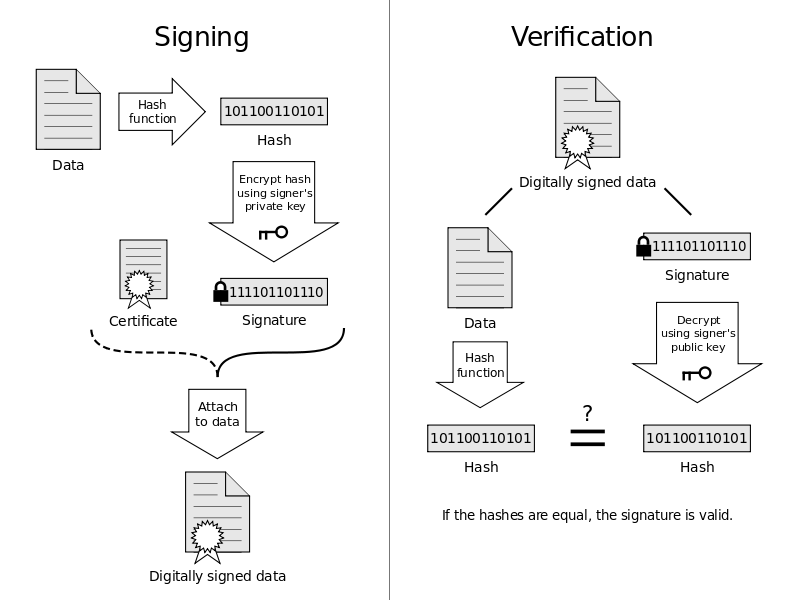
\includegraphics[height=8cm]{crypto5.png}}
\caption{Criação de assinaturas digitais com funções de síntese.}
\label{fig:crypto5}
\end{figure}

O remetente da mensagem cria uma assinatura digital aplicando uma função de síntese (Hash function) no documento (Data), produzindo-se um ficheiro sintetizado (Hash). Este ficheiro é cifrado usando a sua chave privada de forma a produzir uma assinatura digital que é depois anexada ao documento (Digitally signed data). Após a receção do documento assinado, o destinatário decifra a assinatura através da chave pública do assinante e executa uma síntese ao próprio ficheiro. São produzidos dois ficheiros Hash e a verificação consiste em comparar os valores produzidos, i.e., se forem iguais a assinatura é considerada válida.

De referir que no contexto das assinaturas digitais é aplicado um dos objetivos da criptografia moderna: o não-repúdio. Ou seja, o remetente não deverá ser capaz de negar mais tarde que foi realmente a pessoa que enviou a mensagem.

\section{Criptografia Simétrica}
\label{chalp.simétrica}

A cifra simétrica é a forma mais básica de criptografia na qual é partilhada uma chave entre o emissor e o recetor da mensagem, geralmente designada por chave simétrica, e usada por ambos para cifrar e decifrar mensagens. Além de possuírem a mesma chave, os intervenientes também devem possuir o mesmo algoritmo, neste caso designado por algoritmo simétrico. A figura \ref{fig:crypto1} ilustra de forma simples o uso de chave partilhada na realização da criptografia simétrica.

\begin{figure}[ht]
\center
\fbox{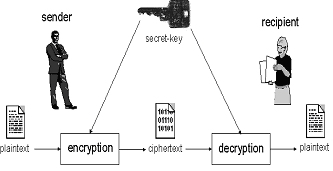
\includegraphics[height=4cm]{crypto1.jpg}}
\caption{Uso de chave simétrica na criptografia simétrica.}
\label{fig:crypto1}
\end{figure}

O remetente (sender) cifra o texto em claro (plaintext) através da chave privada (secret -key), produzindo-se um texto cifrado (ciphertext). O destinatário (recipient) da mensagem decifra-a usando a chave partilhada por ambos. O processo contrário também funciona, ou seja, a chave tanto pode servir para cifrar como para decifrar mensagens.

A criptografia simétrica divide-se em dois tipos de cifras: contínua e por blocos.

\subsection{Cifras Simétricas Contínuas}

Na cifra contínua, a mensagem em claro é tratada como uma sequência de bytes (ou bits) onde cada sequência é cifrada sequencialmente. Usa uma operação relativamente simples para misturar a mensagem original com uma chave contínua pseudo-aleatória de dimensão finita também designada por keystream. Esta operação é tipicamente a função XOR (Exclusive- OR) visto que é uma função facilmente invertível.\\

A operação de cifra consiste em aplicar a função XOR para cada sequência de bytes do texto em claro juntamente com a correspondente sequência de bytes da chave contínua (as sequências também podem ser de 1 bit). A expressão \ref{eq1} mostra como é feita a operação de cifra.

\begin{equation}
\label{eq1}
C = T \oplus Ks
\end{equation}

Onde C é o criptograma, T é o texto em claro e Ks a chave contínua (keystream).\\

A operação de decifra pode ser executada aplicando novamente a função XOR. A expressão \ref{eq2} mostra como é feita a operação de decifra.

\begin{equation}
\label{eq2}
T = C \oplus Ks
\end{equation}

Onde T é o texto em claro, C é o criptograma e Ks a chave contínua (keystream).\\

De referir que é usada a mesma chave nas duas equações \ref{eq1} e \ref{eq2}.

\subsection{Cifras Simétricas por Blocos}

Na cifra por bloco, a mensagem é dividida em blocos de igual dimensão sendo cada um deles processados de forma independente dos restantes. Conforme o algoritmo aplicado para cifrar e decifrar mensagens, os blocos podem ter dimensões diferentes. Por exemplo, o DES (Data Encryption Standard) e o AES (Data Encryption Standard) são dois algoritmos bastante usados neste tipo de cifra, mas, quer um quer outro usam blocos de tamanhos distintos, 64 e 128 bits respetivamente. O criptograma é criado após a criação de vários pequenos criptogramas representando cada um dos blocos cifrados.\\

Um conceito bastante importante neste tipo de cifra é o alinhamento ou padding. Existem modos de cifra por blocos que põem particularmente em prática este conceito. Um deles é o ECB (Electronic Code Book), onde possibilita a separação de ficheiros em blocos de dimensões iguais. Por exemplo, se um determinado ficheiro for separado em blocos e verificar-se que o último não tem uma dimensão igual à dos restantes, é adicionado uma “string” de bytes (ou bits) no final desse bloco de forma a obter o tamanho pretendido. A esse acréscimo de bits dá-se o nome de excipiente, sendo necessário indicar a sua existência e comprimento de forma a facilitar a decifra por parte de quem recebe a mensagem cifrada. A figura \ref{fig:crypto2} ilustra muito basicamente as operações de cifra nas cifras contínuas e por blocos.

\begin{figure}[ht]
\center
\fbox{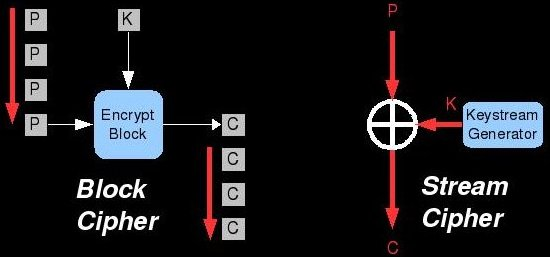
\includegraphics[height=5cm]{crypto2.jpg}}
\caption{Operações de cifra na cifra por blocos (Block Cipher) e contínua (Stream Cipher).}
\label{fig:crypto2}
\end{figure}

Na cifra por blocos, o texto em claro é partido em blocos de dimensões iguais (P1, P2, …, Pn) sendo que cada um deles cifrados de forma independente dos restantes, obtendo-se vários criptogramas (C1, C2, …, Cn) que serão o criptograma. Na cifra contínua, é gerada uma chave contínua e a combinação desta com o texto em claro através da função XOR gera o criptograma (C).

\section{Criptografia Assimétrica}
\label{chap.assimétrica}

A criptografia assimétrica é uma área da criptografia onde cada um dos interlocutores da comunicação tem na sua possessão um par de chaves, uma privada (ou secreta) e outra pública. A chave pública é usada principalmente para cifrar mensagens ou para verificar assinaturas digitais. O termo ‘assimétrico’ vem do facto de se usar duas chaves, mas ambas com funções opostas. A criptografia assimétrica usa cifras por blocos e pode assegurar a confidencialidade e a autenticação nas mensagens transmitidas dependendo de como se usam as chaves e qual para cada situação.\\

Se se pretender comunicar confidencialmente, a chave pública do destinatário é usada para cifrar e a chave privada do destinatário é usada para decifrar, ou seja só o destinatário conseguirá decifrar o criptograma através da sua chave privada. Por outro lado, o destinatário não tem conhecimento de quem remeteu a mensagem cifrada, ou seja, neste caso não há autenticação. A figura \ref{fig:crypto3} ilustra o uso correto das chaves assimétricas para garantir a confidencialidade na transmissão das mensagens entre os interlocutores da comunicação.\\

\begin{figure}[ht]
\center
\fbox{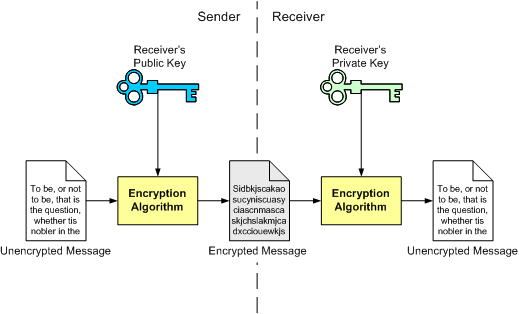
\includegraphics[height=6cm]{crypto3.png}}
\caption{Criptografia assimétrica e confidencialidade.}
\label{fig:crypto3}
\end{figure}

O remetente (sender) deve conhecer a chave pública do destinatário (receiver) para cifrar as suas mensagens e assim comunicar de forma confidencial. O destinatário usa por sua vez a sua chave privada para decifrar o criptograma. Neste caso, só é usado o par de chaves do lado do destinatário.

Por outro lado, se o destinatário pretender garantir a autenticação da origem da mensagem recebida, por exemplo em documentos com assinaturas digitais, as chaves são usadas de forma contrária, ou seja, a chave privada do remetente é usada para cifrar as mensagens. O destinatário decifra o criptograma usando a chave pública do remetente e verifica que foi este último quem gerou o criptograma. Neste caso, não há confidencialidade visto que a chave usada para cifrar é pública (chave pública do remetente), ou seja, quem a conhecer poderá decifrar o criptograma. A figura \ref{fig:crypto4} ilustra a transmissão de mensagens usando chaves assimétricas para garantir a autenticação da origem das mesmas.\\

\begin{figure}[ht]
\center
\fbox{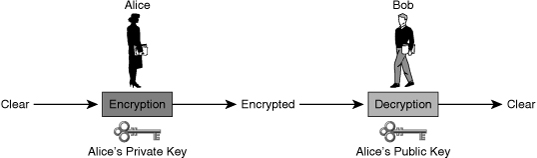
\includegraphics[height=3cm]{crypto4.jpg}}
\caption{Criptografia assimétrica e autenticação.}
\label{fig:crypto4}
\end{figure}

O emissor (Alice) cifra a mensagem através de um algoritmo assimétrico e da sua chave privada (Alice’s Private Key) e envia para o destinatário (Bob). Este, por sua vez, decifra o criptograma através da chave pública do emissor (Alice’s Public Key) verificando a autenticação do autor. Neste caso, só se usa o par de chaves do lado do emissor.

\section{Criptografia Híbrida}
\label{chap.híbrida}

A cifragem híbrida tira partido não só da segurança extra e autenticidade que algoritmos assimétricos permitem, como também da velocidade oferecida por algoritmos simétricos. Assim, procura juntar-se o melhor de um e de outro processos. Assim sendo, o que este método geralmente permite é a cifragem da mensagem a transmitir, que poderá ser um ficheiro bastante grande e onde, portanto, torna-se muito mais proveitoso utilizar um algoritmo simétrico, segundo um metódo de cifram assimétrica. Veja-se um simples exemplo de utilização, em que um certo indivíduo A pretendo enviar uma mensagem cifrada a outro, B (segundo este metódo de cifragem híbrida):
\begin{enumerate}
\item A terá de obter a chave pública de B.
\item Gera-se uma chave simétrica aleatória.
\item Cifra-se a mensagem segundo um algoritmo de cifragem simétrica como AES.
\item A chave simétrica utilizada é cifrada segundo um algoritmo assimétrico (utilizando a chave pública de B)
\item Ambos a mensagem e a chave cifradas são enviados a B.
\end{enumerate}
O que B terá de fazer quando receber os ficheiros, de forma a decifrar a mensagem, deverá ser algo como:
\begin{enumerate}
\item B utiliza a sua chave privada para decifrar a chave simétrica utilizada para cifragem da mensagem.
\item É utilizada essa chave simétrica para decifrar a mensagem enviada.
\end{enumerate}

\chapter{Implementação de Programas}
\label{chap.programas}

Neste capítulo irá ser abordada a implementação de dois programas, um com o objectivo de cifrar e o outro de decifrar uma certa mensagem. Ambos utilizam um esquema híbrido \ref{chap.híbrida}, portanto fornecendo confidencialidade e autenticidade mas permitindo uma rápida cifragem e decifragem da mensagem a ser enviada. Os pares de chaves assimétricas utilizados nos testes destes programas foram gerados utilizando o programa \href{run:../Python/KeysGenerator/generateKeys.py}{\textbf{generateKeys.py}}. O código de ambos os programas é disponibilizado em apêndixe no final deste relatório para facilitar o confronto do código exposto face à análise levada a cabo sobre ele em cada uma das seções seguintes, secções em que se procura explicar como se procurou resolver o problema inicialmente exposto.\\
Para facilitar certas explicações abaixo, parte-se do princípio que que o indivíduo A quer enviar em ficheiro cifrado a B, que só este último pode decifrar, e em que é possível verificar a autenticidade do ficheiro.

\section{Cifragem}

O programa responsável pela cifragem da mensagem a transmitir é \href{run:../Python/Sender/encipherPy.py}{\textbf{encipherPy.py}}. O código do programa é incluido neste relatório em \ref{App:encipher.py}.
Este programa depende de várias funções para sua execução, destancando-se as funções \verb|sigGenerator|, \verb|keyGenerator| e \verb|encipher|. Outras funções nele presentes estão relacionadas com a robustês deste e não com a cifragem da mensagem em si, e portanto não irão ser abordadas.\\
O objectivo deste programa é tirar partido da velocidade de cifram com chaves simétricas, mas manter as funcionalidades e segurança extra que chaves assimétricas permitem. Com isso em mente, em gerada uma chave simétrica pelo programa, que é cifrada com a chave pública de B (para que apenas este a possa decifrar), a assinatura do ficheiro é cifrada com a chave privada de A (para que B possa ter certezas sobre a origem do ficheiro), e o ficheiro em si é cifrado com uma chave simétrica, sendo portanto muito mais rápida a sua cifragem e decifragem.\\
Apesar de nas funções a seguir expostas se falar na criação de ficheiros auziliares (\verb|*.sig| e \verb|*.key|) e dum ficheiro principal \verb|*.bin|, estes não estão presentes no final da execução do programa já que se optou por juntar todos estes ficheiros num único \verb|*.all|, facilitando assim o envio do ficheiro cifrado. Este processo é um dos implementados pelas funções auxiliares referidas acima, não estando relacionado com a cifragem em si.

\subsection{sigGenerator}

Esta função é responsável pela criação de uma assinatura do ficheiro, de forma a garantir ao recetor da mensagem que o que ele está a receber (e decifrar) é de facto a mensagem enviada (ou, no caso de não ser, pelo menos isso será facilmente verificado), e que esta foi enviada pelo indivíduo A.\\
Para isto recorre-se a uma função de síntese, \verb|SHA-256|\footnote{\url{http://en.wikipedia.org/wiki/SHA-2}}, para calcular o \verb|hash| do ficheiro a cifrar. De seguida recorre-se ao módulo \verb|PKCS1_v1_5|\footnote{\url{https://www.dlitz.net/software/pycrypto/api/current/toc-Crypto.Signature.PKCS1_v1_5-module.html}} para gerar uma assinatura com a chave privada de A, sendo esta gravada num ficheiro \verb|*.sig|, onde \verb|*| simboliza o nome do ficheiro original sem extensão.

\subsection{keyGenerator}

Esta função tem como objectivo gerar e guardar a chave simétrica usada pelo programa, cifrando-a com a chave pública de B (de forma a que apenas este a possa decifrar). Para isso, inicialmente gera-se uma sequência aleatória de 1024 bits. Visto que o método de encriptação AES necessita de chaves com 16, 24 ou 32 bytes, é calculada a síntese (SHA-256) do código aleatório gerado de forma a garantir que a chave final é de 256 bits (ou seja, 32 bytes). De seguida esta chave é cifrada com a chave pública de B recorrendo-se ao módulo \verb|PKCS1_OAEP|\footnote{\url{https://www.dlitz.net/software/pycrypto/api/current/toc-Crypto.Cipher.PKCS1_OAEP-module.html}}, garantindo-se assim que apenas B pode decifrar esta chave (com a sua chave privada), obtendo a chave necessária à decifragem da mensagem enviada. O resultado é depois guardado num ficheiro \verb|*.key|, onde mais uma vez \verb|*| simboliza o nome do ficheiro a cifrar sem extensão.\\
Para além da chave cifrada, é também guardado um código IV (Initialization Vector) necessário à correcta descodificação da mensagem. Este código é gerado na função \verb|encipher|, sendo que a função \verb|keyGenerator| apenas o guarda no mesmo ficheiro onde a chave é guardada. Este código é necessário em resultado da utilização do mode de encpritção de AES CFB\footnote{\url{http://goo.gl/RxmaQC}}.

\subsection{encipher}

Por último, processa-se de facto a cifragem do ficheiro recorrendo-se para isso à função \verb|encipher|. Esta implementa as duas funções anteriormente expostas, de forma o obter os resultados nelas exposto. Para além disso, gera também um código de 16 bytes chamado de \verb|iv|\footnote{\url{http://en.wikipedia.org/wiki/Initialization_vector}}, necessário pelo modo de cifragem em uso. Finalmente o ficheiro é cifrado recorrendo-se ao módulo de cifragem AES\footnote{\url{https://www.dlitz.net/software/pycrypto/api/current/toc-Crypto.Cipher.AES-module.html}}, modo CFB, e o resultado é guardado num ficheiro \verb|*.bin|.\\
O recetor da mensagem, indivíduo B, poderá utilizar a sua chave privada para obter a chave simétrica gerada para cifrar este ficheiro. Desta forma tira-se partido da velocidade de cifragem com chaves simétricas, mas mantém-se a segurança extra (e autenticação) que chaves assimétricas permitem.

\section{Decifragem}

A decifragem da mensagem cifrada enviada é feita pelo programa \href{../Python/Receiver/decipherPy.py}{\textbf{decipherPy.py}}\ref{App:decipher.py}. Também este programa recorre essencialmente a três funções para decifrar o ficheiro pedido, possuindo no entanto mais código responsável por aumentar a sua robustez e utilidade. O seu ojectivo é ser capaz de decifrar a chave simétrica utilizada para cifrar a mensagem (com a chave privada do utilizador do programa decifrador, ou seja, com a chave privada do indivíduo B), e com ela decifrar a mensagem inicial. Posto isto, é corrida uma função de verificação que visa garantir não só a integridade do ficheiro como também a sua autenticidade. Para isto, o ficheiro onde foi guardada a assinatura do ficheiro original é decifrado com a chave pública de A (quem envia a mensagem), sendo depois analizada a integridade do ficheiro comparando a sua síntese SHA-256 com a originalmente guardada. De seguida irão ser analizadas em maior detalhe cada uma das funções mais relacionadas com a decifragem do ficheiro.

\subsection{hashVerification}

Esta é a função encarregue de verificar a autenticidade e integridade do ficheiro recebido. Note-se que mesmo que mesmo que a verificação falhe a decifragem prossegue.\\
Para garantir a autenticidade e integridade do ficheiro, quando este foi cifrado foi gerada uma sua assinatura, guardada num ficheiro auxiliar \verb|*.sig|. Desta forma, é agora possível ao utilizador B, por meio do programa \verb|decipherPy.py| inferir sobre a origem deste, bem como se foi ou não adulterado. Para isto, recorre-se novamente ao módulo \verb|PKCS1_v1_5|, em especial à sua função \verb|RSASSA-PKCS1-V1_5-VERIFY|\footnote{\url{http://goo.gl/OPdiHU}} que permite, tal como o nome indica, permite correr as verificações pretendidas.\\
Caso a verificação seja concluida com sucesso será imprimida uma mensagem para o terminal de forma a indicar isso mesmo, acompanhada da síntese SHA-256 do ficheiro. Caso contrário, apenas surgirá uma mensagem indicando que a verificação falhou.

\subsection{keyReader}

Esta função é a que permite a obtenção da chave (de 32 bytes) usada aquando da cifragem simétrica, bem como do código IV (de 16 bytes) utilizado no mesmo processo. Ambas as chaves encontram-se guardadas no ficheiro \verb|*.key|, sendo que a chave de 32 bytes está cifrada com a chave pública do recetor (utilizador B) enquanto que o código de 16 bytes não. De forma a obter ambas estas chaves, o programa lê os primeiros 16 bytes do ficheiro \verb|*.key|, onde o código IV foi guardado, procedendo-se depois à leitura do resto do ficheiro. Este "resto" é depois decifrado com a chave privada de B (recorrendo a \verb|PKCS1_OAEP|), obtendo-se assim a chave simétrica utilizada para cifragem do ficheiro original.

\subsection{decipher}

Esta é a função que permite a verdadeira decifragem do ficheiro (no entanto pelo menos a função \verb|keyReader| é também essencial para que esta decifragem seja possível). Esta decifragem é feita de modo inverso à cifragem feita pela função homóloga \verb|encipher| (do programa de cifragem), e, sendo assim, recorre-se também ao algoritmo AES, modo CFB, com o mesmo valor IV para decifragem do ficheiro. A chave utilizada nesta decifragem é também a mesma para a cifragem (já que estamos perante um algoritmo de cifragem simétrica), e obtida recorrendo-se à função \verb|keyReader|. No final da decifragem, é levada a cabo a verificação do ficheiro final através da função \verb|hashVerification|.\\
No final, o ficheiro decifrado é guardado num ficheiro com o mesmo nome que o indicado para decifragem, sem extensão.

\chapter{Conclusões}
\label{chap.conclusões}

\appendix
\newpage
\section{encipherPy.py} \label{App:encipher.py}

\begin{minted}[frame=lines,fontsize=\footnotesize,linenos]{python}
import os, sys, zipfile
from Crypto import Random
from Crypto.Cipher import AES, PKCS1_OAEP
from Crypto.Hash import SHA256
from Crypto.PublicKey import RSA
from Crypto.Random import random
from Crypto.Signature import PKCS1_v1_5


# Define Public and Private key names!

# Sender's private key:
priKey = "A_PrivateKey.pem"
# Receiver's public key:
pubKey = "B_PublicKey.pem"

# File name to encrypt
f_name = ""

def usage():
    print "python encipherPy.py <File_Name>"


def sigGenerator(priKey_fname, f_name):
    # Opening and reading file to encrypt

    f = open(f_name, "r")
    buffer = f.read()
    f.close()

    # Creating Hash of the file. Using SHA-256 (there was a problem using SHA-512)

    h = SHA256.new(buffer)

    # Reading PrivateKey to sign file with

    keyPair = RSA.importKey(open(priKey_fname, "r").read())
    keySigner = PKCS1_v1_5.new(keyPair)

    # Saving Signature to *.sig File

    f = open(f_name.split('.')[0] + ".sig", "w")
    f.write(keySigner.sign(h))
    f.close()


def keyGenerator(pubKey_fname, f_name, iv):
    # Generating 1024 random bits, and creating SHA-256 (for 32 bits compatibility with AES)

    h = SHA256.new(str(random.getrandbits(1024)))

    # Reading PublicKey to encrypt AES key with

    keyPair = RSA.importKey(open(pubKey_fname, "r").read())
    keyCipher = PKCS1_OAEP.new(keyPair.publickey())

    # Saving encrypted key to *.key File

    f = open(f_name.split('.')[0] + ".key", "w")
    f.write(iv + keyCipher.encrypt(h.digest()))
    f.close()

    # Returning generated key to encrypt file with

    return h.digest()


def encipher(keyA_fname, keyB_fname, f_name):
    # Opening file to encrypt in binary mode

    f = open(f_name, "rb")
    buffer = f.read()
    f.close()

    # Generating file's Signature (and saving it)

    sigGenerator(keyA_fname, f_name)

    # Generating initializing vector for AES Encryption (there were problems when using different AES modes)
    # Needs to be saved in, for example, .key File!!!

    iv = Random.new().read(AES.block_size)

    # Generating symmetric key for use (and saving it)

    k = keyGenerator(keyB_fname, f_name, iv)

    # Encrypting and saving result to *.bin File. Using CFB mode

    keyCipher = AES.new(str(k), AES.MODE_CFB, iv)
    f = open(f_name.split('.')[0] + ".bin", "wb")
    f.write(keyCipher.encrypt(buffer))
    f.close()


def auxFilesZip(sig, key, bin):
    # Opening file to contain all bin, sig and key files

    f = zipfile.ZipFile(bin.split('.')[0] + ".all", "w")

    # Writing each of the arguments to the created file

    f.write(sig)
    f.write(key)
    f.write(bin)

    # Closing the file

    f.close()

    # Running clean up to the bin, sig and key files

    cleanUp(sig, key, bin)


def cleanUp(sig, key, bin):
    # Deleting each of the files generated during ciphering

    os.remove(sig)
    os.remove(key)
    os.remove(bin)


def checkFiles(f_name, pubKey, priKey):
    # Checking for encrypting file's existence and access

    if not os.path.isfile(f_name) or not os.access(f_name, os.R_OK):
        print "Invalid file to encrypt. Aborting..."
        sys.exit(1)

    # Checking for each of the files to create existence and, in case they exist, if they are writable

    else:
        s = f_name.split('.')[0]
        if os.path.isfile(s + ".sig") and not os.access(s + ".sig", os.W_OK):
            print "Can't create temporary file: *.bin. Aborting..."
            sys.exit(2)
        if os.path.isfile(s + ".key") and not os.access(s + ".key", os.W_OK):
            print "Can't create temporary file: *.key. Aborting..."
            sys.exit(3)
        if os.path.isfile(s + ".bin") and not os.access(s + ".bin", os.W_OK):
            print "Can't create temporary file: *.bin. Aborting..."
            sys.exit(4)
        if os.path.isfile(s + ".all") and not os.access(s + ".all", os.W_OK):
            print "Can't create output file. Aborting..."
            sys.exit(5)

    # Checking for public key's existence and access

    if not os.path.isfile(pubKey) or not os.access(pubKey, os.R_OK):
        print "Invalid public key file. Aborting..."
        sys.exit(6)

    # Checking for private key's existence and access

    if not os.path.isfile(priKey) or not os.access(priKey, os.R_OK):
        print "Invalid private key file. Aborting..."
        sys.exit(7)


# Gathering encrypting file name

if len(sys.argv) > 2:
    usage()
elif len(sys.argv) == 1:
    print "File name:"
    f_name = raw_input(">>> ")
else:
    f_name = sys.argv[1]

# Gathering keys names

if priKey == "":
    print "Sender's private key file name:"
    priKey = raw_input(">>> ")
if pubKey == "":
    print "Receiver's public key file name:"
    pubKey = raw_input(">>> ")

# Running checks to files

checkFiles(f_name, pubKey, priKey)

# Ciphering file (and generating all auxiliary files)

encipher(priKey, pubKey, f_name)

# Generating output file and clean up

auxFilesZip(f_name.split('.')[0] + ".sig", f_name.split('.')[0] + ".key", f_name.split('.')[0] + ".bin")
\end{minted}

\newpage
\section{decipherPy.py} \label{App:decipher.py}

\begin{minted}[frame=lines,fontsize=\footnotesize,linenos]{python}
import os, sys, zipfile
from Crypto.Cipher import PKCS1_OAEP, AES
from Crypto.Hash import SHA256
from Crypto.PublicKey import RSA
from Crypto.Signature import PKCS1_v1_5


# Define Public and Private key names!

# Sender's public key:
pubKey = "A_PublicKey.pem"
# Receiver's private key:
priKey = "B_PrivateKey.pem"

# File name to decrypt
f_name = ""

def usage():
    print "python decipherPy.py <File_Name>"


def hashVerification(pubKey_fname, f_name):
    # Generating decrypted file's SHA-256

    h = SHA256.new()
    h.update(open(f_name, "r").read())

    # Reading PublicKey to check Signature with

    keyPair = RSA.importKey(open(pubKey_fname, "r").read())
    keyVerifier = PKCS1_v1_5.new(keyPair.publickey())

    # If Signature is right, prints SHA-256. Otherwise states that the file is not authentic

    if keyVerifier.verify(h, open(f_name.split('.')[0] + ".sig", "r").read()):
        print "The signature is authentic."
        print "SHA-256 -> %s" % h.hexdigest()
    else:
        print "The signature is not authentic."


def keyReader(privKey_fname, f_name):
    # Reading PrivateKey to decipher Symmetric key used

    keyPair = RSA.importKey(open(privKey_fname, "r").read())
    keyDecipher = PKCS1_OAEP.new(keyPair)

    # Reading iv (initializing vector) used to encrypt and saving Symmetric key used to 'k'

    f = open(f_name.split('.')[0] + ".key", "r")
    iv = f.read(16)
    k = keyDecipher.decrypt(f.read())

    return k, iv


def decipher(keyA_fname, keyB_fname, f_name):
    # Getting Symmetric key used and iv value generated at encryption process

    k, iv = keyReader(keyB_fname, f_name)

    # Deciphering the initial information and saving it to file with no extension

    keyDecipher = AES.new(k, AES.MODE_CFB, iv)
    bin = open(f_name + ".bin", "rb").read()
    f = open(f_name.split('.')[0], "wb")
    f.write(keyDecipher.decrypt(bin))
    f.close()

    # Running a Signature verification

    hashVerification(keyA_fname, f_name.split('.')[0])


def auxFilesUnzip(all):
    # Opening the input file

    f = zipfile.ZipFile(all + ".all", "r")

    # Extracting all of its files

    f.extractall()


def cleanUp(sig, key, bin, all):
    # Removing all of the files created, except for the final deciphered file

    os.remove(sig)
    os.remove(key)
    os.remove(bin)
    os.remove(all)

def checkFiles(f_name, pubKey, priKey, first_run):
    # Checking for decrypting file's existence and access

    if first_run and (not os.path.isfile(f_name + ".all") or not os.access(f_name + ".all", os.R_OK)):
        print "Invalid file to decrypt. Aborting..."
        sys.exit(1)

    elif not first_run:
        # Checking if all of the necessary files exist and are accessible

        if not os.path.isfile(f_name + ".sig") or not os.access(f_name + ".sig", os.R_OK):
            print "Invalid *.sig file. Aborting..."
            sys.exit(2)
        if not os.path.isfile(f_name + ".key") or not os.access(f_name + ".key", os.R_OK):
            print "Invalid *.key file. Aborting..."
            sys.exit(3)
        if not os.path.isfile(f_name + ".bin") or not os.access(f_name + ".bin", os.R_OK):
            print "Invalid *.bin file. Aborting..."
            sys.exit(4)

        # Checking if in case of output file's existence, it is writable

        if os.path.isfile(f_name) and not os.access(f_name, os.W_OK):
            print "Can't create output file. Aborting..."
            sys.exit(5)

    # Checking for public key's existence and access

    if not os.path.isfile(pubKey) or not os.access(pubKey, os.R_OK):
        print "Invalid public key file. Aborting..."
        sys.exit(6)

    # Checking for private key's existence and access

    if not os.path.isfile(priKey) or not os.access(priKey, os.R_OK):
        print "Invalid private key file. Aborting..."
        sys.exit(7)


# Gathering encrypting file name

if len(sys.argv) > 2:
    usage()
elif len(sys.argv) == 1:
    print "File name:"
    f_name = raw_input(">>> ")
else:
    f_name = sys.argv[1]

# Gathering keys names

if pubKey == "":
    print "Sender's public key file name:"
    pubKey = raw_input(">>> ")
if priKey == "":
    print "Receiver's private key file name:"
    priKey = raw_input(">>> ")


f_name = f_name.split('.')[0]
checkFiles(f_name, pubKey, priKey, True)
auxFilesUnzip(f_name)
checkFiles(f_name, pubKey, priKey, False)
decipher(pubKey, priKey, f_name)
cleanUp(f_name + ".sig", f_name + ".key", f_name + ".bin", f_name + ".all")
\end{minted}

\maketitle
\nocite{*}
\printbibliography[title={Referências}]

\end{document}
